\documentclass[11pt]{article}
\usepackage[utf8]{inputenc}
\usepackage{graphicx}
\usepackage{hyperref}
\usepackage[a4paper, total={6in, 8in}]{geometry}

\title{Notes on Chapter 10 - Some Simple Algorithms and Data Structures}
\author{Swarup Tripathy \thanks{John V Guttag}}
\date{May 2022}


\begin{document}
    \maketitle
    A curated list of important points for my reference.\\
    \begin{enumerate}
        \item Introduction to Algorithms, by Cormen, Leiserson, Rivest, and Stein, is an excellent source for thous of you not intimidated by a fair amount of mathematics.
        \item The key to efficiency is a good algorithm, not clever coding tricks.
        \item \textbf{SEARCH ALGORITHMS}
        \begin{enumerate}
            \item a method for finding an item or group of items with specific properties within a collection of items.
        \end{enumerate}
        \item \textbf{SORTING ALGORITHMS}
        \begin{itemize}
            \item The standard implementation of sorting in most Python implementations runs in roughly O(n*log(n)) time, where n is the length of the list. 
            \item In most cases, the right thing to do is to use either Python's built in sort method \textit{L.sort()} or its built in function sorted \textit{sorted(L)}
            \item \textit{SELECTION SORT}
            \begin{itemize}
                \item given list [4,2,6,1]
                \item a 'while loop' over individual elements
                \item a 'for loop' under 'while loop' traversing over individual elements
                \item if the 'for loop' element is less than the 'while loop' element, swap it
                \item Here the complexity of the algorithm will be quadratic in the length of L.
            \end{itemize}
            \item \textit{MERGE SORT}
            \begin{itemize}
                \item Also known as Divide and Conquer Algorithm.
                \item Breaks down problem into multiple subproblems recursively until they become simple to solve.
                \item Solutions are combined to solve original problem
                \item O(n*log(n)) is the running time, optimal running time for comparison based algorithms.
                \item General Principle
                \begin{itemize}
                    \item Split array in half
                    \item Call mergeSort on each half to sort them recursively
                    \item Merge both sorted halves into one sorted array. 
                    \item We continue this until we get arrays of size 1, since arrays of size 1 are always sorted.
                    
                    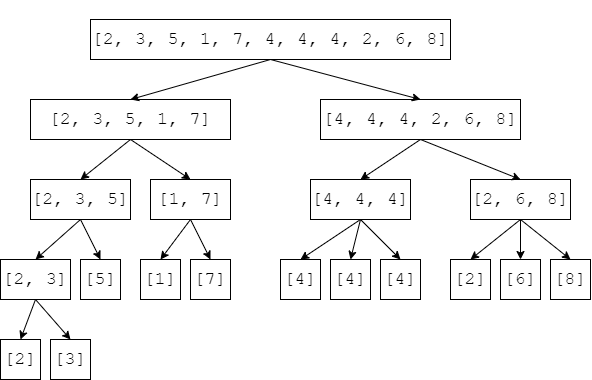
\includegraphics[width=10cm]{07-MergeSort2.drawio.png}

                    \item At the bottom nodes, you can observe arrays of size 1
                \end{itemize}
            \end{itemize}
        \end{itemize}
    \end{enumerate}
\end{document}